% ---------------------------------------------------------------------------
% SNF-Bench -- supplementary material.
%
% Built from the same unmodified author kit as main.tex: same documentclass
% line, same wacv options, same preamble. Nothing in the conference template is
% edited here either; \maketitlesupplementary comes from wacv.sty.
%
% Wide material uses table*/figure* so nothing is cramped or overset.
%
% Compile independently:  tectonic -X compile supp.tex
% ---------------------------------------------------------------------------
\documentclass[10pt,twocolumn,letterpaper]{article}

\usepackage[review,datasets]{wacv}

\usepackage{graphicx}
\usepackage{booktabs}
\usepackage{amsmath}
\usepackage{amssymb}
\usepackage{xcolor}
%
% --- inline annotations
%
\newcommand{\red}[1]{{\color{red}#1}}
\newcommand{\todo}[1]{{\color{red}#1}}
\newcommand{\TODO}[1]{\textbf{\color{red}[TODO: #1]}}
% --- disable by uncommenting  
% \renewcommand{\TODO}[1]{}
% \renewcommand{\todo}[1]{#1}




% --- auto-generated numbers -------------------------------------------------
% Emitted by scripts/paper_assets.py from the frozen scores. Loaded here (and
% again, harmlessly, from main.tex) so that whichever file a build system reads
% first, the macros exist. They use \providecommand, so double loading is safe.
\IfFileExists{generated/macros.tex}{% AUTO-GENERATED by scripts/paper_assets.py -- do not edit.
% Every number the prose quotes lives here, so a score change propagates into the text instead of silently diverging from it.

\newcommand{\SNFdarNegN}{129}
\newcommand{\SNFdarNegPct}{9.6}
\newcommand{\SNFdarTotN}{1345}
\newcommand{\SNFddNBF}{+0.93}
\newcommand{\SNFfeatBackbone}{ORB}
\newcommand{\SNFflowBackbone}{RAFT}
\newcommand{\SNFnCategories}{6}
\newcommand{\SNFnPromptsSixty}{23}
\newcommand{\SNFnPublicTTV}{7}
\newcommand{\SNFrankCFDD}{1}
\newcommand{\SNFrankCFNBF}{7}
\newcommand{\SNFrankCFfBD}{7}
\newcommand{\SNFrankIFDD}{7}
\newcommand{\SNFrankIFNBF}{1}
\newcommand{\SNFrankIFfBD}{1}
\newcommand{\SNFspecVersions}{1.0}
\newcommand{\SNFtopCatShare}{61}
\newcommand{\SNFvalCFDAR}{0.40}
\newcommand{\SNFvalCFDLR}{0.94}
\newcommand{\SNFvalCFNBF}{87.6}
\newcommand{\SNFvalCFfBD}{22.8}
\newcommand{\SNFvalIFDAR}{0.10}
\newcommand{\SNFvalIFDLR}{0.55}
\newcommand{\SNFvalIFNBF}{3.64}
\newcommand{\SNFvalIFfBD}{7.72}
}{%
  \GenericWarning{}{SNF-Bench: generated/macros.tex missing -- run scripts/paper_assets.py}}
\IfFileExists{generated/provenance.tex}{% AUTO-GENERATED provenance

\providecommand{\SNFprovenance}{%
Metrics computed under METRIC\_SPEC v1.0, 1.1 with the RAFT flow backbone and ORB features.}
}{%
  \GenericWarning{}{SNF-Bench: generated/provenance.tex missing -- run scripts/paper_assets.py}}


\definecolor{wacvblue}{rgb}{0.21,0.49,0.74}
\usepackage[pagebackref,breaklinks,colorlinks,allcolors=wacvblue]{hyperref}

\def\wacvPaperID{*****}
\def\confName{WACV}
\def\confYear{2027}

\title{SNF-Bench: Separating Static Drift from Natural Flow in Long-Horizon Fixed-Camera Video Generation}

\begin{document}
\maketitlesupplementary

\IfFileExists{generated/macros.tex}{% AUTO-GENERATED by scripts/paper_assets.py -- do not edit.
% Every number the prose quotes lives here, so a score change propagates into the text instead of silently diverging from it.

\newcommand{\SNFdarNegN}{129}
\newcommand{\SNFdarNegPct}{9.6}
\newcommand{\SNFdarTotN}{1345}
\newcommand{\SNFddNBF}{+0.93}
\newcommand{\SNFfeatBackbone}{ORB}
\newcommand{\SNFflowBackbone}{RAFT}
\newcommand{\SNFnCategories}{6}
\newcommand{\SNFnPromptsSixty}{23}
\newcommand{\SNFnPublicTTV}{7}
\newcommand{\SNFrankCFDD}{1}
\newcommand{\SNFrankCFNBF}{7}
\newcommand{\SNFrankCFfBD}{7}
\newcommand{\SNFrankIFDD}{7}
\newcommand{\SNFrankIFNBF}{1}
\newcommand{\SNFrankIFfBD}{1}
\newcommand{\SNFspecVersions}{1.0}
\newcommand{\SNFtopCatShare}{61}
\newcommand{\SNFvalCFDAR}{0.40}
\newcommand{\SNFvalCFDLR}{0.94}
\newcommand{\SNFvalCFNBF}{87.6}
\newcommand{\SNFvalCFfBD}{22.8}
\newcommand{\SNFvalIFDAR}{0.10}
\newcommand{\SNFvalIFDLR}{0.55}
\newcommand{\SNFvalIFNBF}{3.64}
\newcommand{\SNFvalIFfBD}{7.72}
}{%
  \GenericWarning{}{SNF-Bench: generated/macros.tex missing}}
\IfFileExists{generated/provenance.tex}{% AUTO-GENERATED provenance

\providecommand{\SNFprovenance}{%
Metrics computed under METRIC\_SPEC v1.0, 1.1 with the RAFT flow backbone and ORB features.}
}{%
  \GenericWarning{}{SNF-Bench: generated/provenance.tex missing}}

\noindent
This supplement records the material supporting the main paper without being
required to follow its argument: the region-partition procedure and its
sensitivity study, complete audit tables for both tracks at every horizon,
measurement coverage, protocols for the two complementary perceptual checks, and
additional qualitative material. The text-conditioned and image-conditioned
tracks are reported here at equal depth. Section numbering is independent of the
main paper.

\section{Formal Factor Definitions}
\label{sup:defs}

The definitions below are those referenced from the main paper's protocol
section. Notation follows it: $I_t$ is frame $t$ of a $T$-frame sequence,
$\Omega_{\mathrm{static}}$ and $\Omega_{\mathrm{flow}}$ are the region masks,
$\mathbf{u}_t$ is the optical flow from $I_t$ to $I_{t+1}$, and $\mathcal{E}$
and $\mathcal{L}$ are the early and late windows.

\paragraph{Feature-aligned Background Drift.}
For matched ORB pairs $\mathcal{M}_t$ between the first frame and frame $t$,
\begin{align}
D_{\mathrm{feat}}(t) &= \operatorname*{median}_{(p,q)\in\mathcal{M}_t} \lVert p-q \rVert_2, \nonumber\\
\mathrm{fBD} &= \frac{100}{d}\cdot\frac{1}{|\mathcal{L}|}\sum_{t\in\mathcal{L}} D_{\mathrm{feat}}(t) \;\;(\downarrow),
\end{align}
with $d$ the frame diagonal, so fBD is a percentage of image size.

\paragraph{Normalised Background Flow.}
\begin{equation}
\mathrm{NBF} = \frac{10^3}{W\,\Delta t}\cdot\frac{1}{T-1}\sum_{t=1}^{T-1}
\frac{1}{|\Omega_{\mathrm{static}}|}\sum_{\mathbf{x}\in\Omega_{\mathrm{static}}}
\lVert \mathbf{u}_t(\mathbf{x}) \rVert_2
\;\;(\downarrow),
\end{equation}
with $W$ the frame width and $\Delta t$ the interval of the \emph{sampled} pairs
actually used for flow estimation, so the quantity is independent of both the
native frame rate and the sampling policy.

\paragraph{Global-motion compensation.}
With $T_t(\mathbf{x}) = s_t R_t \mathbf{x} + \mathbf{b}_t$ the robust similarity
transform fitted to static-region correspondences and
$\mathbf{d}_t(\mathbf{x}) = T_t(\mathbf{x})-\mathbf{x}$ the displacement field it
induces,
\begin{equation}
\tilde{\mathbf{u}}_t(\mathbf{x}) = \mathbf{u}_t(\mathbf{x}) - \mathbf{d}_t(\mathbf{x}).
\end{equation}

\paragraph{Motion-Compensated Foreground Flow and Flow Persistence.}
\begin{equation}
\mathrm{MCFF}(\mathcal{W}) = \frac{1}{|\mathcal{W}|}\sum_{t\in\mathcal{W}}
\frac{1}{|\Omega_{\mathrm{flow}}|}\sum_{\mathbf{x}\in\Omega_{\mathrm{flow}}}
\lVert \tilde{\mathbf{u}}_t(\mathbf{x}) \rVert_2
\;\;(\uparrow),
\end{equation}
\begin{equation}
\mathrm{FP} = \min\!\left(\frac{\mathrm{MCFF}(\mathcal{L})}{\mathrm{MCFF}(\mathcal{E})+\epsilon},\, c\right)
\;\;(\uparrow),
\end{equation}
clipped at a fixed $c$ so that a vanishing early window cannot produce an
unbounded ratio.

\paragraph{Drift leakage and attenuation.}
With $F_{\mathrm{static}}$ the mean flow magnitude over $\Omega_{\mathrm{static}}$
and $F_{\mathrm{raw}}$, $F_{\mathrm{comp}}$ the mean raw and compensated
magnitudes over $\Omega_{\mathrm{flow}}$, all in the late window,
\begin{equation}
\mathrm{DLR} = \frac{F_{\mathrm{static}}}{F_{\mathrm{raw}}+\epsilon}\;\;(\downarrow),
\qquad
\mathrm{DAR} = 1 - \frac{F_{\mathrm{comp}}}{F_{\mathrm{raw}}+\epsilon}\;\;(\downarrow).
\end{equation}
DLR is not a fraction and is deliberately unbounded: $\mathrm{DLR}>1$ indicates
static support moving more than the region intended to move. DAR is stored
signed and reported clipped to $[0,1]$.

\section{Region Partition}
\label{sup:masks}

\paragraph{Derivation.}
For every generated sequence we average optical-flow magnitude~\cite{teed2020raft}
over the leading $12\%$ of sampled frame pairs and threshold it by Otsu's
method~\cite{otsu1979threshold} into a dynamic region and its complement. The
static region is then reduced by a fixed morphological erosion and a $4\%$ frame
border discarded; together these form the ignored transition band, so boundary
pixels---where the partition is least certain and flow least reliable---contribute
to neither region. The same procedure applies to both tracks.

\paragraph{Why the estimate is restricted to an early window.}
Deriving a partition from a sequence's entire motion field would be circular,
since accumulated background drift would itself be read as evidence that the
affected region is dynamic. Restricting the estimate to the early window breaks
that circularity in the direction that matters: at the $60$\,s horizon the
partition is fixed from the first $7.1$\,s, before long-horizon drift has
accumulated, and the metrics are evaluated over the remainder.

\paragraph{Limitations.}
The partition is obtained automatically rather than by annotation, so no
inter-annotator agreement is reported, and for the image-conditioned track it is
derived per generated sequence rather than once from the shared source image.
The early window is a weaker guarantee than a first-frame annotation: a system
that drifts within the first $12\%$ of its rollout can influence its own
partition. We therefore treat partitions as measured quantities and report the
consequence directly---every measurement is recomputed under systematic erosion
and dilation of the boundary, with the response in Table~\ref{tab:validation}.

\begin{figure}[tb]
\centering
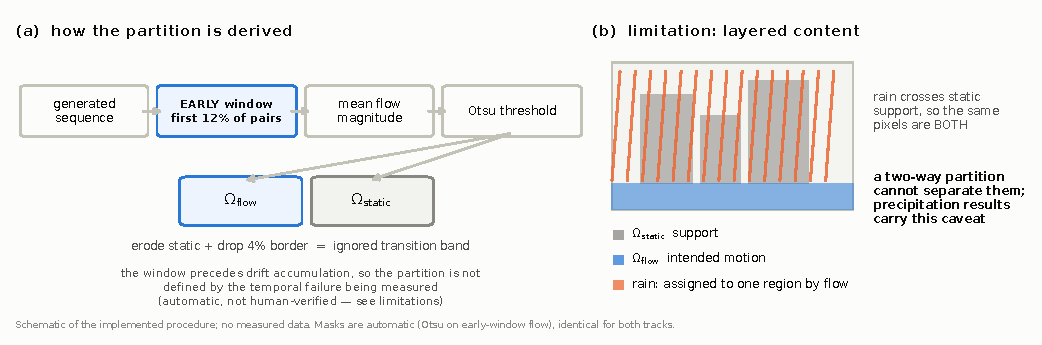
\includegraphics[width=\linewidth]{figures/fig2_mask_protocol.pdf}
\caption{\textbf{Region-partition protocol.} (a)~The partition is derived automatically from early-window flow, with an ignored transition band at the boundary. (b)~A two-way partition cannot represent layered content such as rain crossing static support, which is the scope limit stated in the main paper.}
\label{sup:fig_mask}
\end{figure}

\section{Validation Protocol}
\label{sup:validation}

Geometric severity is specified in a common physical unit---the mean pixel
displacement a corruption induces over the frame by the end of the
rollout---and each family's parameter is derived from it using the frame
geometry: a translation of $d$ pixels, a rotation of $d/\bar{r}$ radians, or a
zoom of $1 + d/\bar{r}$, where $\bar{r}$ is the mean distance from the frame
centre. This is what makes the geometric families comparable. A parameter in
degrees is not commensurate with one in pixels: at the evaluation resolution one
degree of rotation induces roughly $2.7$\,px of mean displacement, so families
compared by their native parameters differ in injected severity by more than an
order of magnitude, and a factor can appear non-monotone simply because the
corruption was too weak to clear the clip's own baseline drift.

\begin{table}[t]
\centering
\small
\setlength{\tabcolsep}{3.5pt}
\begin{tabular}{l cccccccc}
\toprule
perturbation & clips & fBD & NBF & MCFF-L & FP & DLR & DAR & VB-DD \\
\midrule
translation & 2 & +1.00 & +1.00 & -0.90 & -0.30 & +0.50 & +0.90 & +0.90 \\
rotation & 2 & -0.30 & +1.00 & -0.30 & +0.60 & +0.70 & +0.40 & +0.10 \\
scale & 2 & +0.70 & +0.20 & -1.00 & +0.00 & -0.20 & +0.10 & +0.60 \\
attenuation & 2 & -0.87 & -1.00 & -1.00 & -1.00 & +0.40 & -0.70 & -1.00 \\
freeze & 2 & +1.00 & +1.00 & +1.00 & +1.00 & -0.80 & +0.40 & +1.00 \\
\bottomrule
\end{tabular}
\caption{\textbf{Mechanistic validation.} Spearman correlation between injected severity and each factor's response, over controlled perturbations of real fixed-camera clips. Signs are fixed in advance by each definition. \emph{mask radius} perturbs the region partition rather than the video, so near-zero entries indicate the desired insensitivity. Cells where a factor responds weakly or non-monotonically are reported rather than omitted.}
\label{tab:validation}
\end{table}

\section{Generation Configuration}
\label{sup:config}

Every audited system was run in its released configuration. What the run
manifest records is reported below; what it does not record is stated rather
than reconstructed. Per-method sampler settings---denoising steps, chunk
length, guidance scale, cache policy---were not captured at generation time,
and we do not infer them after the fact. This is the weakest point in the
reproducibility of the audit, and it constrains what the results support: they
compare the systems as released and run here, not the space of settings each
admits.

\begin{table*}[tb]
\centering
\small
\setlength{\tabcolsep}{5pt}
\begin{tabular}{l l c c l}
\toprule
System & setting & resolution & fps & horizons \\
\midrule
CausVid & native & 832$\times$480 & 16 & 5s, 60s, 120s, 240s \\
Self-Forcing & native & 832$\times$480 & 16 & 5s, 60s, 120s, 240s \\
Infinite-Forcing & native & 832$\times$480 & 16 & 5s, 60s, 120s, 240s \\
Rolling-Forcing & native & 832$\times$480 & 16 & 5s, 60s, 120s, 240s \\
Reward-Forcing & native & 832$\times$480 & 16 & 5s, 60s, 120s, 240s \\
LongLive & native & 832$\times$480 & 16 & 5s, 60s, 120s, 240s \\
Causal-Forcing & native & 832$\times$480 & 16 & 5s, 60s, 120s, 240s \\
\bottomrule
\end{tabular}
\caption{\textbf{Recorded generation configuration.} Every audited system was run in its released configuration and produced output at the same resolution and frame rate over the same horizons, so no comparison in this paper is confounded by output format. Per-method sampler settings---denoising steps, chunk length, guidance scale, cache policy---were not captured in the run manifest and are therefore not listed here; this is a reproducibility gap we state rather than fill by inference.}
\label{tab:native_config}
\end{table*}

\section{Measurement Coverage}
\label{sup:coverage}

Coverage is counted from valid per-video measurements rather than from the
presence of a results file, so a run that terminated early is reported as
partial. Separately, fBD is feature-based~\cite{rublee2011orb} and declines to
report where too few repeatable keypoints survive; those abstentions are
tabulated rather than folded silently into a smaller $n$.

\begin{table}[tb]
\centering
\scriptsize
\begin{tabular}{llccc}
\toprule
track & horizon & measured & fBD abstained & rate \\
\midrule
I2V & 120s & 400 & 0 & 0.0\% \\
I2V & 240s & 65 & 0 & 0.0\% \\
I2V & 5s & 180 & 0 & 0.0\% \\
I2V & 60s & 630 & 7 & 1.1\% \\
T2V & 120s & 42 & 0 & 0.0\% \\
T2V & 240s & 28 & 0 & 0.0\% \\
T2V & 5s & 48 & 0 & 0.0\% \\
T2V & 60s & 185 & 0 & 0.0\% \\
\bottomrule
\end{tabular}
\caption{\textbf{Measurement coverage and fBD abstention.} fBD is feature-based and declines to report when too few repeatable keypoints survive in the static region. Every abstention in this benchmark occurs on a single desert dust-storm scene, whose flat, dust-obscured ground offers no stable structure to track, and it occurs there for every system alike---so it reflects the scene, not a method. The remaining factors are reported for those clips as usual; only fBD is withheld.}
\label{tab:abstention}
\end{table}
\begin{table*}[!htbp]
\centering
\scriptsize
\setlength{\tabcolsep}{5pt}
\begin{tabular}{lcccccc}
\toprule
Method & status & setting & 5s & 60s & 120s & 240s \\
\midrule
CausVid & public & native & V6 T6 B & V23 T23 B & V6 T6 B & V4 T4 B \\
Self-Forcing & public & native & V6 T6 B & V23 T23 B & V6 T6 B & V4 T4 B \\
Infinite-Forcing & public & native & V6 T6 B & V23 T23 B & V6 T6 B & V4 T4 B \\
Rolling-Forcing & public & native & V6 T6 B & V24 T24 B & V6 T6 B & V4 T4 B \\
Reward-Forcing & public & native & V12 T12 B & V23 T23 B & V6 T6 B & V4 T4 B \\
LongLive & public & native & V6 T6 B & V23 T23 B & V6 T6 B & V4 T4 B \\
Causal-Forcing & public & native & V6 T6 B & V23 T23 B & V6 T6 B & V4 T4 B \\
\bottomrule
\end{tabular}
\caption{Asset and score coverage for the audited public systems. \texttt{T$n$/$N$} marks entries where a metrics file exists but only $n$ of $N$ videos hold usable measurements.}
\label{tab:coverage}
\end{table*}

\section{Complete Audit, Both Tracks}
\label{sup:allhorizons}

The main paper reports the text-conditioned track at $60$\,s, the tier whose
sample supports method-level separation. Both tracks appear here at every
horizon, with uncertainty from a percentile bootstrap over
items~\cite{efron1979bootstrap}. For the image-conditioned track, systems marked
\emph{matched} run under a common long-horizon wrapper rather than their
released configuration, so their scores are read as deployment sensitivity
rather than as the published method's performance.

\begin{table*}[t]
\centering
\small
\setlength{\tabcolsep}{4pt}
\begin{tabular}{l l cccccccc}
\toprule
Method & setting & $n$ & fBD$\downarrow$ & NBF$\downarrow$ & MCFF-E & MCFF-L$\uparrow$ & FP$\uparrow$ & DLR$\downarrow$ & DAR$\downarrow$ \\
\midrule
\multicolumn{10}{l}{\textit{60s horizon}} \\
CausVid & native & 23 & 8.08 & 9.27 & 2.87 & 1.96 & 0.67 & 0.45 & 0.14 \\
Self-Forcing & native & 23 & 11.4 & 12.7 & 10.4 & 2.54 & 0.44 & 0.50 & 0.14 \\
Infinite-Forcing & native & 23 & 7.75 & 3.65 & 1.17 & 0.29 & 0.63 & 0.55 & 0.14 \\
Rolling-Forcing & native & 23 & 16.8 & 11.2 & 3.18 & 1.57 & 0.75 & 0.54 & 0.18 \\
Reward-Forcing & native & 23 & 14.8 & 8.51 & 3.81 & 0.80 & 0.49 & 0.60 & 0.17 \\
LongLive & native & 23 & 15.9 & 13.9 & 6.46 & 2.41 & 0.75 & 0.59 & 0.17 \\
Causal-Forcing & native & 23 & 22.4 & 87.6 & 9.84 & 7.21 & 0.83 & 0.94 & 0.43 \\
\midrule
\multicolumn{10}{l}{\textit{240s horizon}} \\
CausVid & native & 4 & 7.23 & 13.4 & 0.42 & 0.87 & 0.99 & 0.85 & 0.08 \\
\bottomrule
\end{tabular}
\caption{\textbf{Complete T2V audit, all horizons.} Main-paper Table~\ref{tab:t2v_audit} reproduces the 60\,s and 120\,s panels.}
\label{tab:t2v_audit_full}
\end{table*}
\begin{table*}[t]
\centering
\small
\setlength{\tabcolsep}{4pt}
\begin{tabular}{l l cccccccc}
\toprule
Method & setting & $n$ & fBD$\downarrow$ & NBF$\downarrow$ & MCFF-E & MCFF-L$\uparrow$ & FP$\uparrow$ & DLR$\downarrow$ & DAR$\downarrow$ \\
\midrule
\multicolumn{10}{l}{\textit{5s horizon}} \\
Causal-Forcing++ (2-step) & matched & 10 & 3.69 & 10.0 & -- & 0.65 & 0.88 & 0.67 & 0.22 \\
Causal-Forcing++ (1-step) & matched & 10 & 5.28 & 11.4 & -- & 0.51 & 0.66 & 0.66 & 0.24 \\
Causal-Forcing (framewise) & matched & 10 & 16.1 & 45.3 & -- & 3.28 & 0.40 & 0.68 & 0.12 \\
Causal-Forcing++ (2-step, native nfpb=1) & native & 10 & 1.22 & 10.6 & -- & 0.83 & 0.49 & 0.68 & 0.11 \\
Self-Forcing & matched & 10 & 9.66 & 5.74 & -- & 0.33 & 0.65 & 0.74 & 0.07 \\
CausVid & matched & 10 & 15.2 & 10.8 & -- & 0.90 & 0.95 & 1.04 & 0.06 \\
Wan2.1-I2V-14B-480P & native & 10 & 5.01 & 21.3 & -- & 4.84 & 1.03 & 0.52 & 0.16 \\
Wan2.2-I2V-A14B & native & 10 & 6.31 & 25.3 & -- & 9.08 & 0.95 & 0.50 & 0.26 \\
LTX-Video 13B-0.9.8-distilled & native & 10 & 6.65 & 17.8 & -- & 3.68 & 0.90 & 0.39 & 0.18 \\
\midrule
\multicolumn{10}{l}{\textit{60s horizon}} \\
Causal-Forcing++ (2-step) & matched & 30 & 9.18 & 5.97 & -- & 0.67 & 0.86 & 0.67 & 0.15 \\
Causal-Forcing++ (1-step) & matched & 30 & 5.34 & 7.05 & -- & 0.65 & 0.77 & 0.64 & 0.16 \\
Causal-Forcing (framewise) & matched & 1 & 23.4 & 50.5 & -- & 1.57 & 0.65 & 0.87 & 0.30 \\
Causal-Forcing++ (2-step, native nfpb=1) & native & 30 & 9.94 & 6.91 & -- & 0.81 & 0.98 & 0.75 & 0.11 \\
Self-Forcing & matched & 30 & 17.3 & 5.52 & -- & 0.74 & 0.88 & 0.67 & 0.14 \\
CausVid & matched & 1 & 24.9 & 1.45 & -- & 0.11 & 0.66 & 0.59 & 0.03 \\
Causal-Forcing++ (1-step, native) & native & 30 & 10.4 & 5.25 & -- & 0.52 & 0.97 & 0.83 & 0.14 \\
\midrule
\multicolumn{10}{l}{\textit{120s horizon}} \\
Causal-Forcing++ (2-step) & matched & 20 & 9.65 & 8.81 & -- & 0.93 & 0.91 & 0.58 & 0.14 \\
Causal-Forcing++ (1-step) & matched & 20 & 7.26 & 9.39 & -- & 0.83 & 0.84 & 0.62 & 0.16 \\
Causal-Forcing (framewise) & matched & 1 & 19.4 & 16.7 & -- & 0.99 & 1.59 & 0.86 & 0.31 \\
Causal-Forcing++ (2-step, native nfpb=1) & native & 20 & 11.4 & 17.3 & -- & 1.54 & 0.96 & 0.75 & 0.06 \\
Self-Forcing & matched & 20 & 23.0 & 10.3 & -- & 0.78 & 0.44 & 0.66 & 0.20 \\
CausVid & matched & 1 & 20.7 & 2.57 & -- & 0.20 & 0.89 & 0.61 & 0.00 \\
Causal-Forcing++ (1-step, native) & native & 20 & 13.6 & 7.39 & -- & 0.43 & 0.68 & 0.77 & 0.20 \\
\midrule
\multicolumn{10}{l}{\textit{240s horizon}} \\
Causal-Forcing++ (2-step) & matched & 5 & 10.4 & 4.83 & -- & 0.63 & 1.03 & 0.55 & 0.09 \\
Causal-Forcing++ (1-step) & matched & 1 & 0.98 & 3.58 & -- & 0.12 & 0.39 & 0.86 & 0.40 \\
Causal-Forcing (framewise) & matched & 5 & 19.8 & 31.5 & -- & 2.86 & 0.76 & 0.69 & 0.33 \\
Causal-Forcing++ (2-step, native nfpb=1) & native & 5 & 6.32 & 3.95 & -- & 0.69 & 0.66 & 0.83 & 0.01 \\
Self-Forcing & matched & 5 & 22.3 & 5.74 & -- & 1.66 & 0.79 & 0.71 & 0.05 \\
CausVid & matched & 5 & 18.4 & 2.08 & -- & 0.83 & 0.83 & 0.44 & 0.07 \\
\bottomrule
\end{tabular}
\caption{\textbf{Complete I2V audit, all horizons.} Main-paper Table~\ref{tab:i2v_audit} reproduces the 60\,s and 120\,s panels.}
\label{tab:i2v_audit_full}
\end{table*}

\begin{figure}[tb]
\centering
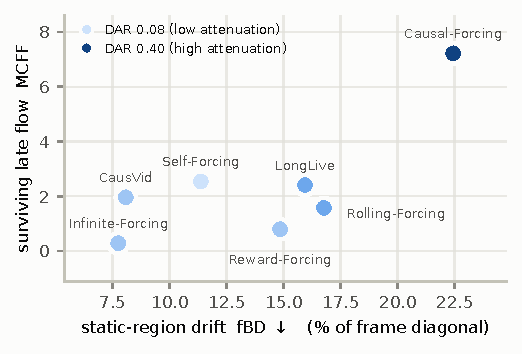
\includegraphics[width=\linewidth]{figures/fig4_operating_regime.pdf}
\caption{\textbf{Operating regimes under native deployment.} Each system in the static-drift--surviving-flow plane. Colour encodes the relative attenuation of measured dynamic-region flow after global-motion compensation, not a share of it attributable to drift: the quantity is signed, and values are shown clipped to $[0,1]$. The view exposes trade-offs; it is not a leaderboard.}
\label{sup:fig_regimes}
\end{figure}

\section{Aggregation Sensitivity}
\label{sup:aggregation}

The evaluation set is dominated by one flow medium, so the audit must be shown
not to be a report on that medium alone. The main paper aggregates by averaging
over prompts. The alternative, weighting each scene category equally, is not
preferable here: at the principal horizon three of the five populated categories
contain two prompts each, so a macro-average would give a two-prompt cell the
same influence as a fourteen-prompt one and inflate variance in exchange for
nominal balance. We therefore report both and state what changes.

The best- and worst-ranked systems are the same under either aggregation, so the
contrast the paper draws does not depend on the choice. Intermediate ranks do
move, which is why no ordinal claim is made about the middle of the field.

\begin{table*}[tb]
\centering
\small
\setlength{\tabcolsep}{5pt}
\begin{tabular}{l c c c c}
\toprule
System & prompt mean & rank & macro mean & rank \\
\midrule
\multicolumn{5}{l}{\emph{NBF}} \\
\quad Infinite-Forcing & 3.65 & 1 & 4.12 & 1 \\
\quad Reward-Forcing & 8.51 & 2 & 10.11 & 4$^{\dagger}$ \\
\quad CausVid & 9.27 & 3 & 9.93 & 3 \\
\quad Rolling-Forcing & 11.23 & 4 & 11.32 & 5$^{\dagger}$ \\
\quad Self-Forcing & 12.72 & 5 & 8.98 & 2$^{\dagger}$ \\
\quad LongLive & 13.86 & 6 & 14.69 & 6 \\
\quad Causal-Forcing & 87.62 & 7 & 61.70 & 7 \\
\multicolumn{5}{l}{\emph{fBD}} \\
\quad Infinite-Forcing & 7.75 & 1 & 6.10 & 1 \\
\quad CausVid & 8.08 & 2 & 9.51 & 3$^{\dagger}$ \\
\quad Self-Forcing & 11.37 & 3 & 9.27 & 2$^{\dagger}$ \\
\quad Reward-Forcing & 14.85 & 4 & 15.61 & 5$^{\dagger}$ \\
\quad LongLive & 15.94 & 5 & 14.93 & 4$^{\dagger}$ \\
\quad Rolling-Forcing & 16.77 & 6 & 18.85 & 6 \\
\quad Causal-Forcing & 22.44 & 7 & 23.49 & 7 \\
\bottomrule
\end{tabular}
\caption{\textbf{Sensitivity of the audit to category aggregation.} Prompt means, as reported in the main paper, against category macro-averages, for the two static-fidelity factors at the principal horizon. $^{\dagger}$ marks a system whose rank changes. The best- and worst-ranked systems are identical under both, so the paper's headline contrast does not depend on the choice; intermediate positions do change, which is why no ordinal claim is made about the middle of the field.}
\label{tab:aggregation}
\end{table*}

\section{Whole-Frame and SNF-Bench Rank Correlation}
\label{sup:disagreement}

\begin{table}[t]
\centering
\small
\begin{tabular}{lcccc}
\toprule
generic metric & fBD & NBF & MCFF & DLR \\
\midrule
VB-DD & +0.75 & +0.93 & +0.89 & +0.36 \\
VB-bg & -0.64 & -0.71 & -0.75 & -0.50 \\
VB-smooth & -0.96 & -0.82 & -0.61 & -0.64 \\
VB-flick & -0.96 & -0.82 & -0.61 & -0.64 \\
\bottomrule
\end{tabular}
\caption{\textbf{Rank disagreement at 60\,s.} Spearman correlation between generic whole-frame metrics and SNF-Bench factors over method-level means. A positive correlation between apparent motion and background flow is the effect the benchmark isolates.}
\label{tab:disagreement}
\end{table}
\begin{table*}[t]
\centering
\small
\begin{tabular}{l l l p{0.35\textwidth}}
\toprule
Method & Generic evidence & SNF-Bench evidence & Interpretation \\
\midrule
CausVid & VB-DD rank 6/7 & NBF rank 3/7, MCFF-L rank 4/7 & stable sequence with decaying intended motion \\
Causal-Forcing & VB-DD rank 1/7 & NBF rank 7/7, MCFF-L rank 1/7 & high apparent motion accompanied by high static-region motion under the common wrapper \\
Infinite-Forcing & VB-DD rank 7/7 & NBF rank 1/7, MCFF-L rank 7/7 & stable sequence with decaying intended motion \\
LongLive & VB-DD rank 3/7 & NBF rank 6/7, MCFF-L rank 3/7 & high apparent motion accompanied by high static-region motion under the common wrapper \\
Reward-Forcing & VB-DD rank 5/7 & NBF rank 2/7, MCFF-L rank 6/7 & stable sequence with decaying intended motion \\
Self-Forcing & VB-DD rank 2/7 & NBF rank 5/7, MCFF-L rank 2/7 & high apparent motion accompanied by high static-region motion under the common wrapper \\
\bottomrule
\end{tabular}
\caption{\textbf{Interpretation changes between generic whole-frame metrics and SNF-Bench at 60\,s.} Neither evaluation is labeled correct; the table identifies information hidden by whole-frame aggregation. Cases are selected by a fixed rank-gap rule applied to all public methods, so none can be selectively omitted.}
\label{tab:interpretation_changes}
\end{table*}

\section{Deployment Sensitivity}
\label{sup:deployment}

\begin{table*}[tb]
\centering
\small
\setlength{\tabcolsep}{6pt}
\begin{tabular}{l c c c c c}
\toprule
Checkpoint & horizon & $\Delta$fBD & $\Delta$NBF & $\Delta$MCFF-L & $\Delta$DLR \\
\midrule
Causal-Forcing++ (2-step) & 5s & +2.47 & -0.61 & -0.17 & -0.01 \\
Causal-Forcing++ (2-step) & 60s & -0.76 & -0.95 & -0.17 & -0.08 \\
Causal-Forcing++ (2-step) & 120s & -1.71 & -8.46 & -0.73 & -0.17 \\
Causal-Forcing++ (2-step) & 240s & +4.06 & +0.88 & -0.09 & -0.28 \\
Causal-Forcing++ (1-step) & 60s & -5.05 & +1.80 & +0.05 & -0.20 \\
Causal-Forcing++ (1-step) & 120s & -6.34 & +2.00 & +0.31 & -0.14 \\
\bottomrule
\end{tabular}
\caption{\textbf{Deployment sensitivity.} Change from each checkpoint's own released setting to the common long-horizon wrapper, for the two checkpoints evaluated both ways. Absolute wrapper scores are never read as the published method's performance.}
\label{tab:deployment_sensitivity}
\end{table*}

\section{Signed Drift Attenuation}
\label{sup:dar}

Drift attenuation is stored signed and reported clipped to $[0,1]$. Negative
values are informative rather than anomalous: where local flow opposes the
estimated global field, compensation increases the measured magnitude. We report
their incidence rather than suppressing it.

\begin{table*}[tb]
\centering
\scriptsize
\setlength{\tabcolsep}{5pt}
\begin{tabular}{lcccccc}
\toprule
Method & track & dur & n & negative & rate & most negative \\
\midrule
CausVid & i2v & 120s & 20 & 1 & 5.0\% & -0.055 \\
CausVid & i2v & 240s & 5 & 0 & 0.0\% & 0.041 \\
CausVid & i2v & 5s & 10 & 5 & 50.0\% & -1.076 \\
CausVid & i2v & 60s & 30 & 2 & 6.7\% & -0.084 \\
Causal-Forcing++ (1-step) & i2v & 120s & 20 & 1 & 5.0\% & -0.027 \\
Causal-Forcing++ (1-step) & i2v & 240s & 5 & 0 & 0.0\% & 0.175 \\
Causal-Forcing++ (1-step) & i2v & 5s & 10 & 0 & 0.0\% & 0.055 \\
Causal-Forcing++ (1-step) & i2v & 60s & 30 & 0 & 0.0\% & 0.013 \\
Causal-Forcing (frame-wise) & i2v & 120s & 20 & 3 & 15.0\% & -0.171 \\
Causal-Forcing (frame-wise) & i2v & 240s & 5 & 0 & 0.0\% & 0.206 \\
Causal-Forcing (frame-wise) & i2v & 5s & 10 & 0 & 0.0\% & 0.067 \\
Causal-Forcing (frame-wise) & i2v & 60s & 30 & 0 & 0.0\% & 0.008 \\
Causal-Forcing++ (2-step) & i2v & 120s & 20 & 0 & 0.0\% & 0.016 \\
Causal-Forcing++ (2-step) & i2v & 240s & 5 & 0 & 0.0\% & 0.109 \\
Causal-Forcing++ (2-step) & i2v & 5s & 10 & 1 & 10.0\% & -0.164 \\
Causal-Forcing++ (2-step) & i2v & 60s & 30 & 0 & 0.0\% & 0.008 \\
Causal-Forcing++ (1-step, frame-wise) & i2v & 120s & 20 & 0 & 0.0\% & 0.051 \\
Causal-Forcing++ (1-step, frame-wise) & i2v & 60s & 30 & 3 & 10.0\% & -1.420 \\
Causal-Forcing++ (2-step, frame-wise) & i2v & 120s & 20 & 5 & 25.0\% & -0.241 \\
Causal-Forcing++ (2-step, frame-wise) & i2v & 240s & 5 & 1 & 20.0\% & -0.651 \\
Causal-Forcing++ (2-step, frame-wise) & i2v & 5s & 10 & 1 & 10.0\% & -0.288 \\
Causal-Forcing++ (2-step, frame-wise) & i2v & 60s & 30 & 1 & 3.3\% & -0.001 \\
LTX-Video 13B-0.9.8-distilled & i2v & 5s & 10 & 2 & 20.0\% & -0.018 \\
Self-Forcing & i2v & 120s & 20 & 2 & 10.0\% & -0.046 \\
Self-Forcing & i2v & 240s & 5 & 1 & 20.0\% & -0.136 \\
Self-Forcing & i2v & 5s & 10 & 0 & 0.0\% & 0.064 \\
Self-Forcing & i2v & 60s & 30 & 4 & 13.3\% & -0.578 \\
Wan2.1-I2V-14B-480P & i2v & 5s & 10 & 1 & 10.0\% & -0.255 \\
Wan2.2-I2V-A14B & i2v & 5s & 10 & 1 & 10.0\% & -0.335 \\
CausVid & t2v & 120s & 6 & 0 & 0.0\% & 0.047 \\
CausVid & t2v & 240s & 4 & 1 & 25.0\% & -0.384 \\
CausVid & t2v & 5s & 6 & 2 & 33.3\% & -0.093 \\
CausVid & t2v & 60s & 23 & 0 & 0.0\% & 0.005 \\
Causal-Forcing & t2v & 120s & 6 & 0 & 0.0\% & 0.175 \\
Causal-Forcing & t2v & 240s & 4 & 0 & 0.0\% & 0.158 \\
Causal-Forcing & t2v & 5s & 6 & 2 & 33.3\% & -0.273 \\
Causal-Forcing & t2v & 60s & 23 & 3 & 13.0\% & -0.640 \\
Infinite-Forcing & t2v & 120s & 6 & 0 & 0.0\% & 0.023 \\
Infinite-Forcing & t2v & 240s & 4 & 1 & 25.0\% & -0.158 \\
Infinite-Forcing & t2v & 5s & 6 & 0 & 0.0\% & 0.031 \\
Infinite-Forcing & t2v & 60s & 23 & 4 & 17.4\% & -0.359 \\
LongLive & t2v & 120s & 6 & 1 & 16.7\% & -1.076 \\
LongLive & t2v & 240s & 4 & 0 & 0.0\% & 0.022 \\
LongLive & t2v & 5s & 6 & 1 & 16.7\% & -0.139 \\
LongLive & t2v & 60s & 23 & 2 & 8.7\% & -0.051 \\
Reward-Forcing & t2v & 120s & 6 & 1 & 16.7\% & -0.116 \\
Reward-Forcing & t2v & 240s & 4 & 0 & 0.0\% & 0.002 \\
Reward-Forcing & t2v & 5s & 12 & 2 & 16.7\% & -0.145 \\
Reward-Forcing & t2v & 60s & 23 & 3 & 13.0\% & -0.317 \\
Rolling-Forcing & t2v & 120s & 6 & 3 & 50.0\% & -0.353 \\
Rolling-Forcing & t2v & 240s & 4 & 0 & 0.0\% & 0.043 \\
Rolling-Forcing & t2v & 5s & 6 & 1 & 16.7\% & -0.068 \\
Rolling-Forcing & t2v & 60s & 24 & 2 & 8.3\% & -0.038 \\
Self-Forcing & t2v & 120s & 6 & 2 & 33.3\% & -0.130 \\
Self-Forcing & t2v & 240s & 4 & 1 & 25.0\% & -0.153 \\
Self-Forcing & t2v & 5s & 6 & 1 & 16.7\% & -0.046 \\
Self-Forcing & t2v & 60s & 23 & 4 & 17.4\% & -1.117 \\
\bottomrule
\end{tabular}
\caption{Incidence of negative DAR, i.e.\ clips where global-motion compensation \emph{increased} measured dynamic-region flow.}
\label{tab:darneg}
\end{table*}

\section{Evaluation-Set Composition}
\label{sup:categories}

\begin{table*}[tb]
\centering
\scriptsize
\setlength{\tabcolsep}{5pt}
\begin{tabular}{lc}
\toprule
category & definition \\
\midrule
river\_stream & channel water: rivers, streams, creeks, canals, waterfalls, rapids, floods \\
ocean\_waves & open water with wave action: surf, tides, coastal swell, seascapes \\
precipitation & falling water or ice: rain, snowfall, and the surfaces they wet \\
fire\_smoke & combustion plumes: wildfire, campfire, hearth, urban fire, grill smoke \\
lava\_volcanic & volcanic flow and ejecta: lava channels, ash columns, eruption smoke \\
windborne & air-carried particulates and wind-driven vegetation: dust, sand, blossom, leaves, thrashing trees, drifting cloud \\
track/duration & n \\
i2v/5s & 10 \\
i2v/60s & 30 \\
i2v/120s & 20 \\
i2v/240s & 5 \\
t2v/5s & 6 \\
t2v/60s & 23 \\
t2v/120s & 6 \\
t2v/240s & 4 \\
track & source \\
i2v & meta \\
t2v & keyword \\
t2v & keyword-body \\
t2v & override \\
track & duration \\
t2v & 60s \\
\bottomrule
\end{tabular}
\caption{Scene-category balance of the evaluation set, by track and horizon.}
\label{tab:category}
\end{table*}

\section{Preliminary Perceptual Validation of the Factor Axes}
\label{sup:perceptual}

This section asks one question: do independent judges order clip pairs the way
the factors do? It is metric validation, not method preference. Nothing here
ranks systems, and no result from it enters any factor, table or figure
elsewhere in this work. Framed that way a small sample is survivable, because
the object under test is a measurement instrument rather than a leaderboard.

\paragraph{Questions.}
One forced choice per axis, with an explicit third option:
\emph{static stability}---in which clip does the background stay more fixed in
place---and \emph{motion persistence}---in which clip does the intended motion
keep going rather than fade or freeze. Judges are never asked which output is
better, or which looks more natural. ``Better'' conflates the two failures the
benchmark separates, and naturalness is outside the stated scope, so either
question would produce a result the paper could not own.

\paragraph{Pairs.}
A pair is two systems' outputs on the \emph{same prompt at the same horizon},
never across prompts. Pairs are stratified by the relative gap in the axis's own
factor: \emph{clear-gap} pairs, where the factor separates the two outputs, carry
the agreement claim, while \emph{near-tie} pairs test the opposite property---that
where the factors do not separate, judges also cannot tell the clips apart.
Presentation side is randomised per trial and resolved back to a system
identity only after the response is recorded; system names are never shown.

\paragraph{Statistics.}
The unit of analysis is the pair, majority-voted across raters, and intervals
are percentile bootstrap resampling \emph{pairs}. Responses are clustered inside
rater and inside pair, so an interval computed over responses would claim
precision the design does not have. We report inter-rater agreement so the
reader can see whether the raters are signal or noise, and we run no
significance test the sample cannot power: the claim is descriptive agreement,
and saying so plainly is preferable to a $p$-value that would not survive
scrutiny.

\begin{table*}[tb]
\centering
\small
\setlength{\tabcolsep}{6pt}
\begin{tabular}{l l c c c c}
\toprule
Axis & Judge & agrees with factor & called indistinguishable & pairs & inter-rater $\alpha$ \\
\midrule
Static stability (fBD) & human & -- (3 decided) & -- & 8 & 0.18 \\
 & vision--language & -- (1 decided) & 1/1 & 7 & -- \\
Motion persistence (MCFF-L) & human & 80\% {\footnotesize [40, 100]} & -- & 8 & 0.24 \\
 & vision--language & -- (2 decided) & -- & 3 & -- \\
\bottomrule
\end{tabular}
\caption{\textbf{Preliminary perceptual validation of the factor axes.} Each judge answers one question per axis and never which output is better. \emph{agree} is agreement with the factor's ordering on pairs the factor separates clearly, over pairs the judge decided; \emph{can't tell} is the share of near-tie pairs called indistinguishable, which is the correct answer there. The unit is the pair, majority-voted across raters, and the interval is a percentile bootstrap resampling pairs rather than responses, which are clustered within rater and pair. A dash marks a cell with too few decided pairs to carry a rate; the count is given instead. This is a preliminary check on a measurement instrument, not a powered study, and no system is ranked by it.}
\label{tab:perception}
\end{table*}

\paragraph{Outcome of the human arm: the instrument works, agreement is not yet estimable.}
Eight raters each completed all $24$ trials, four of them independent of the
authors; the remaining four were pilot sessions and are reported separately
rather than pooled. Engagement was genuine---median deliberation ran from $23$
to $233$ seconds per trial---and the ``can't tell'' option was used
deliberately, on $30\%$ of responses, rather than avoided.

The agreement estimate, however, does not survive its own error bars. Majority
voting across raters leaves three decided pairs on the static axis and five on
the persistence axis, and the corresponding intervals span most of the unit
range. Inter-rater agreement is low ($\alpha = 0.18$ and $0.24$ on the two
axes), and the direction of the estimate reverses depending on which rater
subset is used. We therefore report the counts and the interval rather than a
headline percentage, and we do not claim that perceptual agreement has been
established.

The cause is a property of the pair set rather than of the raters, and it is
measurable. The pairs were stratified by the gap in each axis's \emph{own}
factor but were not isolated against the other axis. On the static question the
median relative gap in the target factor is $0.29$ while the median gap in the
persistence factor is $0.58$: the clips shown differ about twice as much on the
axis the rater was told to ignore as on the one being asked about, and on half
the pairs both axes differ substantially. A rater seeing one clip drift and the
other stall cannot report which axis drove the answer, which is exactly the
condition that produces low inter-rater agreement and near-chance ordering. A
powered study therefore requires axis-isolated pairs---large gap in the target
factor, small gap in the other---and that constraint, not rater count, is the
first thing to fix.

\paragraph{Outcome of the vision--language arm: negative, with a located cause.}
The same pairs and the same wording were put to an open-weight
judge~\cite{qwen3vl2025} at temperature zero, each pair asked in both
presentation orders. Two controls precede any reading of its answers. Shown one
clip against itself, where the only correct answer is that they are the same, it
answered correctly on six of six. Shown a frozen single frame against a real
sequence---the largest difference available on the motion axis---its verdict
followed the swapped clip on only two of six. Presentation bias is absent: over
$48$ queries the two slots were chosen $8$ and $12$ times. The judge is
therefore well behaved and still cannot do the task: it answered
``indistinguishable'' on most pairs the factors separate clearly, leaving one
and two decided pairs on the two axes, which is far too few to support an
agreement rate. We report none.

The controls locate the cause in the judge rather than in the factors or the
prompt. A model that cannot separate a still image from moving water is not
positioned to separate two rollouts that differ subtly. This says that an
open-weight judge at this scale cannot presently substitute for human raters on
these axes. It does not say that stronger judges would fail, and we make no
claim about them: contemporary generation benchmarks that report successful
automated judging use frontier proprietary
models~\cite{han2025videobench,sun2024t2v_compbench} or scorers fine-tuned for
the task~\cite{he2024videoscore}, and we have no evidence either way about those
here.

\paragraph{Status.}
Both arms are reported as preliminary and neither supports an agreement claim.
What the pilot does establish is that the instrument runs end to end, that
raters engage with the axis questions rather than defaulting to a side, and
that the binding constraint on a powered study is pair construction rather than
rater count: axis-isolated pairs, a near-tie stratum, and raters recruited
outside the authors. Protocol, pair manifest and judge prompt are released
verbatim so the check can be repeated and enlarged.

\section{Additional Qualitative Material}
\label{sup:qualitative}

\begin{figure*}[tb]
\centering
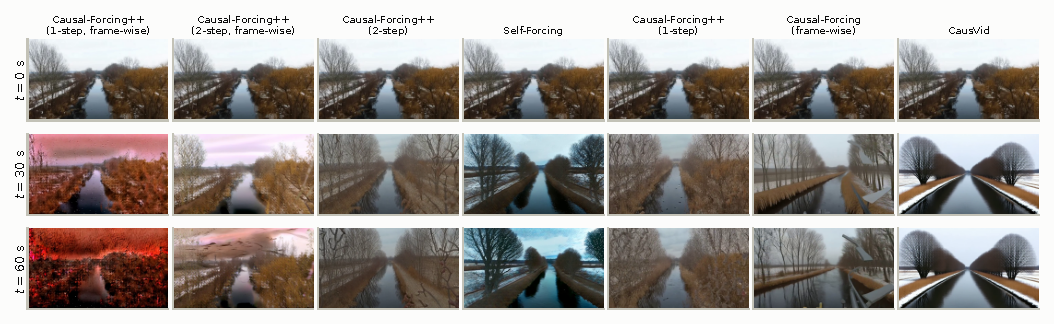
\includegraphics[width=\textwidth]{figures/fig8_i2v_qualitative.pdf}
\caption{\textbf{Image-conditioned systems on one shared source image.} Every
system begins from the identical frame, so divergence over the rollout is
attributable to the system rather than to a differently imagined scene---which
is not true of the text-conditioned track, where each system authors its own
layout. Columns are ordered by increasing static-region drift.}
\label{sup:fig_i2v}
\end{figure*}

\begin{figure*}[tb]
\centering
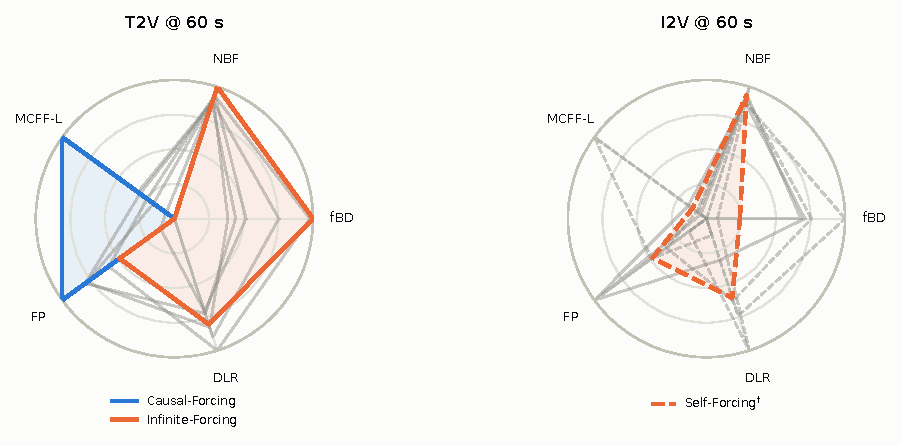
\includegraphics[width=\textwidth]{figures/figS_radar.pdf}
\caption{\textbf{Factor profile per track.} Each factor is rescaled across the
audited systems and oriented so that outward is always better; plotting raw
values would place ``most drift'' and ``most surviving motion'' both outward and
the shape would carry no meaning. No system encloses the others on either track,
which is the conclusion the operating-regime view reaches, shown as a profile.}
\label{sup:fig_radar}
\end{figure*}

\begin{figure*}[tb]
\centering
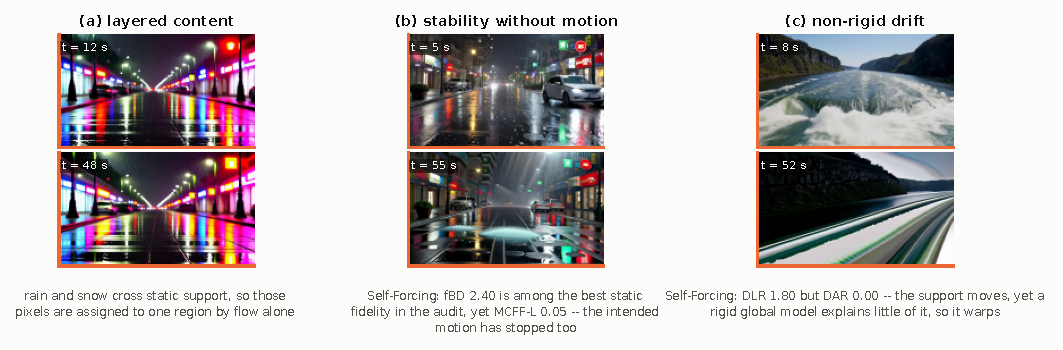
\includegraphics[width=\textwidth]{figures/fig7_limitations.pdf}
\caption{\textbf{Stated scope boundaries.} (a)~A two-way partition cannot
separate precipitation from the support it crosses. (b)~A system can attain
near-best static fidelity precisely because its intended motion has also
stopped. (c)~High leakage with low attenuation identifies support that moves
without translating, which a rigid global model does not explain.}
\label{sup:fig_limits}
\end{figure*}

\begin{figure*}[tb]
\centering
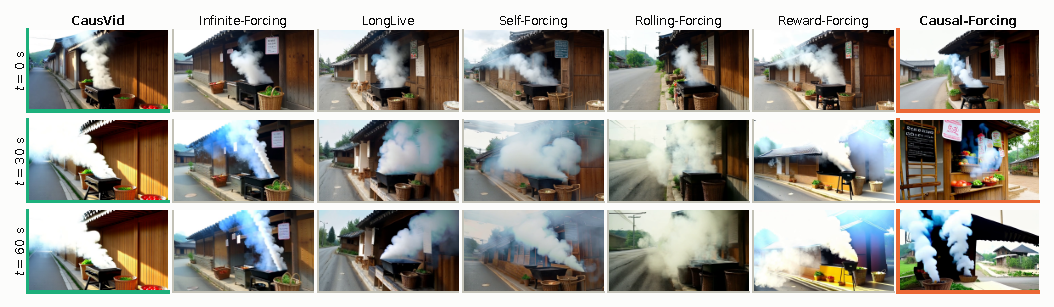
\includegraphics[width=\textwidth]{figures/fig6_qualitative.pdf}
\caption{\textbf{Every audited text-conditioned system on one prompt.} Columns
are ordered by increasing static-region drift; the two highlighted systems are
the pair a whole-frame motion score cannot separate.}
\label{sup:fig_qualitative}
\end{figure*}

\begin{figure*}[tb]
\centering
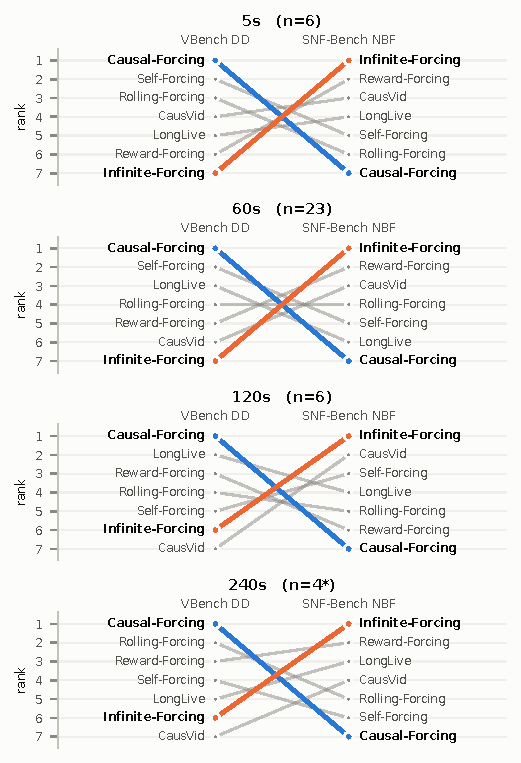
\includegraphics[width=\textwidth]{figures/fig5_rank_disagreement.pdf}
\caption{\textbf{Rank disagreement at every audited horizon.} Rank under a
whole-frame motion score against rank under normalised background flow. Both
quantities are independent of the global-motion estimator; prompt counts are
given per panel.}
\label{sup:fig_ranks}
\end{figure*}

\begin{figure*}[tb]
\centering
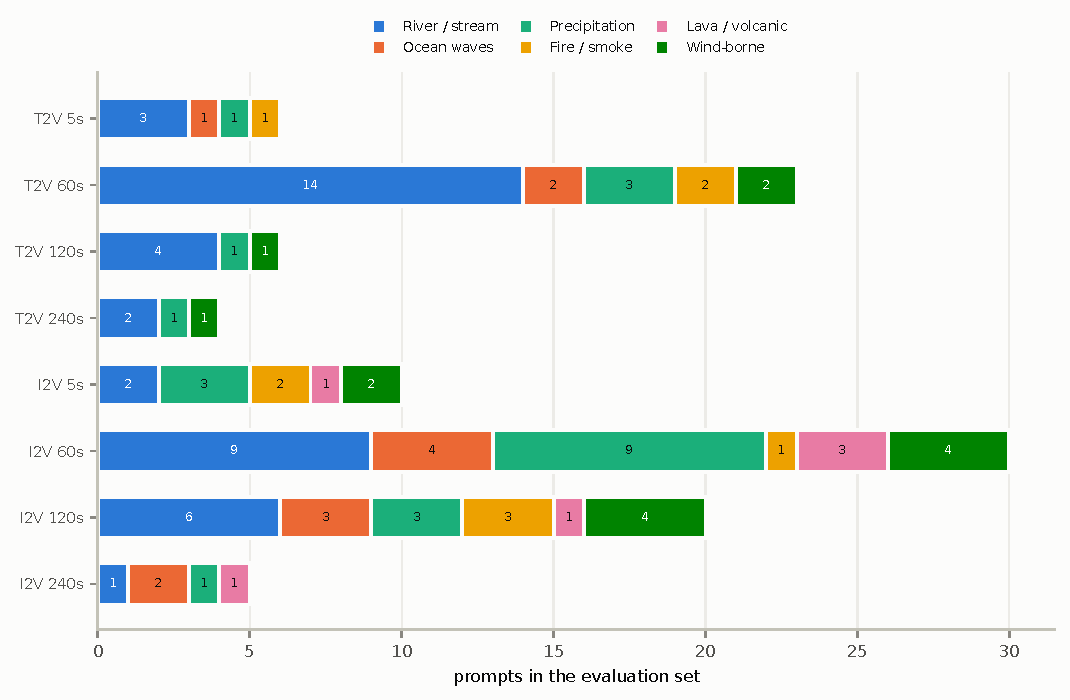
\includegraphics[width=\textwidth]{figures/figS_category_balance.pdf}
\caption{\textbf{Composition of the evaluation set by scene category,} in
prompts per category at each track and horizon.}
\label{sup:fig_categories}
\end{figure*}

{
    \small
    \bibliographystyle{ieeenat_fullname}
    \bibliography{main}
}

\end{document}
